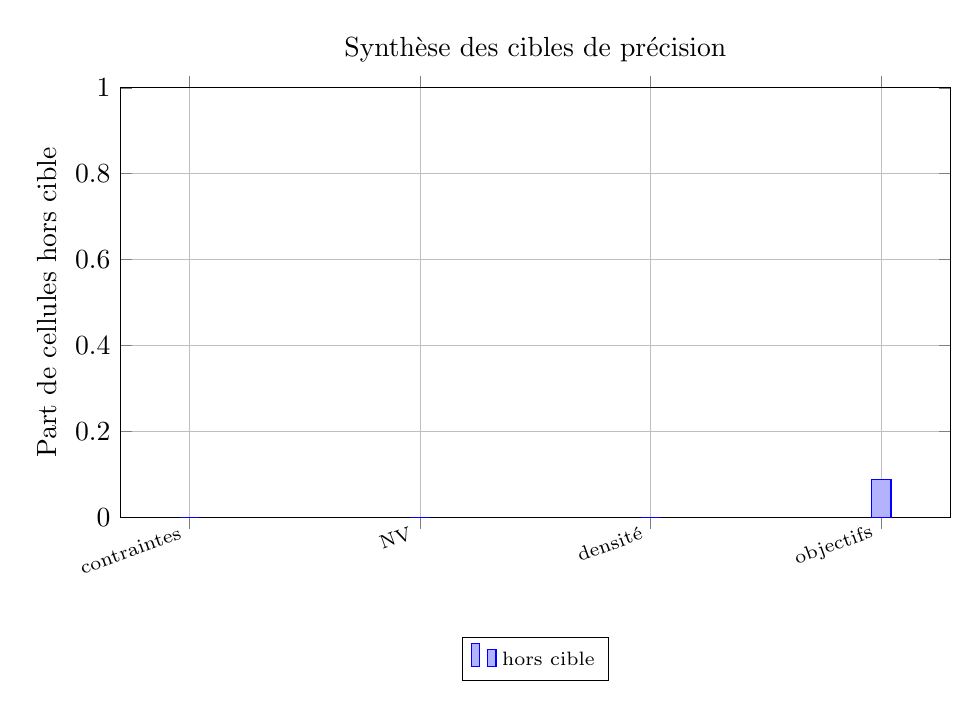
\begin{tikzpicture}
\begin{axis}[ybar,
bar width=7pt,
width=\linewidth,
height=0.58\linewidth,
title={Synthèse des cibles de précision},
ylabel={Part de cellules hors cible},
xtick={0,1,2,3},
xticklabels={{contraintes},{NV},{densité},{objectifs}},
x tick label style={rotate=20,anchor=east,font=\scriptsize},
grid=major,
legend style={font=\scriptsize,at={(0.5,-0.28)},anchor=north,legend columns=1},
ymin=0,
ymax=1.0]
\addplot+ coordinates {(0,0.0) (1,0.0) (2,0.0) (3,0.08854166666666667)};
\addlegendentry{hors cible}
\end{axis}
\end{tikzpicture}
